\section{Related Work} \label{sect_relatedworks}

\subsection{Federated Learning and Intrusion Detection Systems (IDS)}
Federated Learning (FL) has been widely adopted in security-sensitive applications, particularly for building Intrusion Detection Systems (IDS) in distributed IoT and edge environments. By allowing multiple clients to collaboratively train a global model without sharing raw data, FL preserves privacy while leveraging diverse datasets \cite{kairouz2021advances,Nguyen2022}. However, the same decentralization that makes FL attractive also increases its vulnerability to adversarial manipulation. For IDS, where the correctness of anomaly detection is crucial, poisoned updates from a few compromised clients can significantly degrade detection accuracy or even implant backdoors for stealthy intrusions \cite{Liu2020}. Recent advances, such as Fed-LSAE \cite{FedLSAE}, highlight a shift toward latent-space inspection for FL-based IDS, leveraging feature representations instead of raw parameters to enhance robustness against internal poisoning.


\subsection{Model Poisoning Attack}
Among the threats to FL, model poisoning attacks are particularly dangerous. Unlike data poisoning, which corrupts training inputs, model poisoning directly manipulates gradients or weight updates. Attack vectors include sign-flipping, Gaussian perturbations, and label-flipping, as well as more sophisticated strategies such as Little is Enough (LIE), backdoors, and stealthy scaling attacks \cite{fang2020local,Bhagoji2019,baruch2019}. These methods enable adversaries to either degrade global accuracy (untargeted Byzantine attacks) or inject malicious behavior into the global model (targeted backdoors). In Non-IID settings typical of IDS deployments, benign clients naturally produce divergent updates, making it even harder to distinguish between malicious and honest contributions \cite{Shejwalkar2021}.


\subsection{Secured Aggregation and Defense Mechanisms}
To counter poisoning, a broad range of defenses have been proposed. Passive approaches, such as FedMP \cite{ZHAO2025110990}, FL-Guardian \cite{11003999}, DPAD \cite{BASAK2025109893}, and MSGuard \cite{10942405}, rely on anomaly detection or clustering of submitted updates. While effective in controlled settings, they incur high computational overhead and often assume majority honesty, which is fragile under Non-IID distributions. Proactive defenses, such as RECESS \cite{10851419}, introduce active probes (e.g., gradient traps) but remain sensitive to adaptive attackers. Cryptographic methods, including TMT-FL \cite{10812212}, guarantee data integrity through zero-knowledge proofs or blockchain auditing, yet their costs are prohibitive and they do not directly detect semantic poisoning. More recent multi-layer defenses (e.g., FedAMM \cite{11175562}, FedCleanse \cite{HUANG2025114494}, UDFed \cite{Sun2023}, Time-Series Defense \cite{Li2025}) combine multiple signals such as reputation, gradient decomposition, or temporal anomaly detection. In parallel, Fed-LSAE \cite{FedLSAE} introduces a lightweight latent-space inspection defense that filters clients via penultimate-layer representations, Autoencoder compression, and RBF-CKA clustering to exclude malicious participants, yet it assumes a minority of attackers and a fixed configuration. While these strategies improve robustness, they remain limited by scalability, high computational costs, or lack of proactive verification. 


\begin{figure*}[ht]
  \centering
  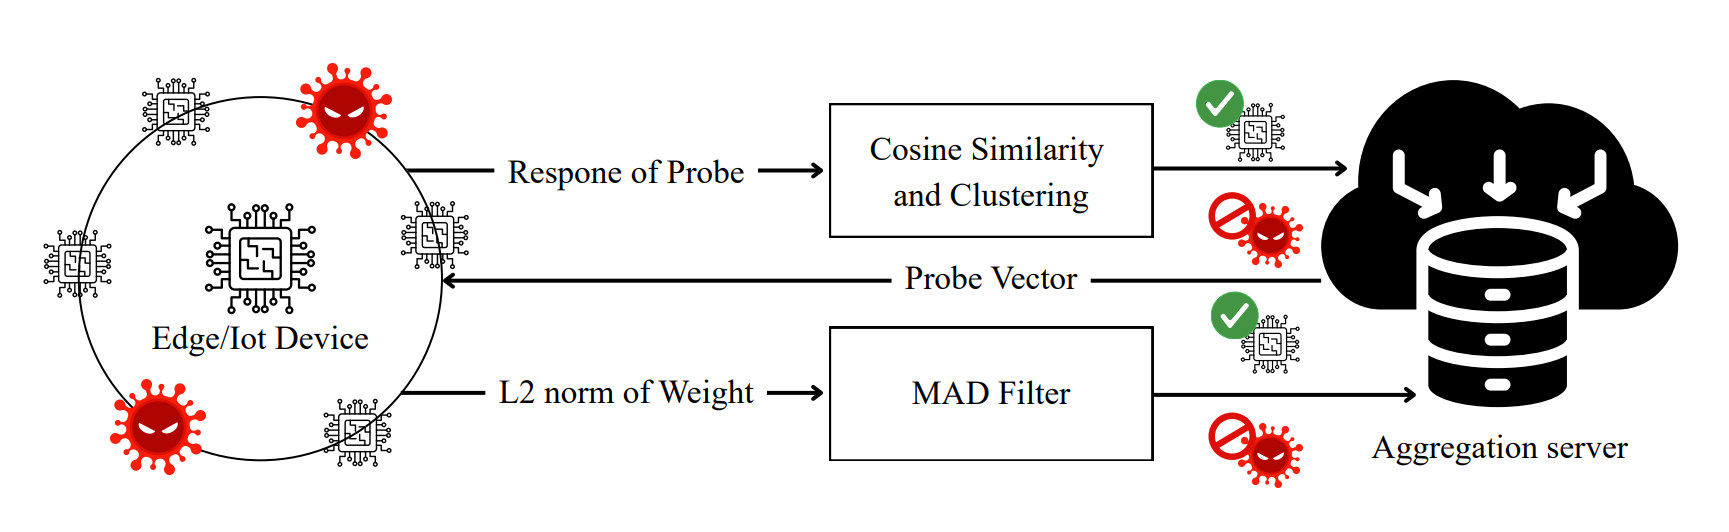
\includegraphics[width=1\linewidth]{images/overview.png}
  \caption{Overview of the proposed Defense Mechanism.}
  \label{fig:framework}
\end{figure*}

\subsection{Non-IID Issues}
A fundamental limitation across most defenses is the Non-IID nature of federated datasets. IDS clients often monitor highly heterogeneous traffic patterns, leading to natural divergence of updates. Defenses that assume benign clients converge toward a majority direction (e.g., MSGuard, FL-Guardian) misclassify honest but divergent clients as adversaries, increasing false positives. Conversely, adaptive attackers can exploit this heterogeneity to camouflage poisoned updates \cite{Shejwalkar2021,Fu2022}. Furthermore, most defenses evaluate updates independently at each round, without considering temporal consistency, leaving them vulnerable to stealthy or slow poisoning \cite{fang2020local}. Fed-LSAE \cite{FedLSAE} alleviates some Non-IID variance through Autoencoder-compressed latent representations but performs round-wise filtering without temporal adaptation.


In light of these challenges, a new defense mechanism must (i) remain lightweight for deployment in edge-based IDS, (ii) operate without clean validation datasets, (iii) adapt to Non-IID environments, and (iv) incorporate temporal analysis to detect stealthy adversaries. Our proposed P4P framework directly addresses these requirements by leveraging probe vectors and temporal chaining in a proactive multi-layer design.

\subsection{Pipeline Overview}

As summarized in Table~\ref{tab:compare}, existing defenses either incur
high computational costs, rely on clean validation data, or fail to handle
Non-IID scenarios effectively. In contrast, our proposed P4P framework
achieves low overhead, strong Non-IID robustness, and temporal resilience,
making it a lightweight yet proactive multi-layer defense.




